\pagebreak
\chapter{Algorithm of learning}
\label{chapter:Algorithm}



\section{Formulation of reinforcement learning}

\subsection{Introduction of Markov decision process}

Normally, reinforcement learning is formulated by a Markov decision process. The Markov decision process(MDP) means that
It models Agents that make decisions and is formulated as a set of four with the following elements.
\begin{itembox}[l]{Markov decision model}
\bm{State:} \hspace{1.2cm} $S = \{ s^{(1)}, s^{(2)}, ... , s^{(N)} \}$

\bm{Action:} \hspace{1cm} $A = \{ a^{(1)}, a^{(2)}, ... , a^{(K)} \}$ 

\bm{Dynamics:} \hspace{5mm} $T : S \times A \times S \rightarrow [0, 1]$ \hspace{1cm} $T(s',a,s) = p(s' | s,a)$

\bm{Reward:} \hspace{0.9cm} $R : S \times A \times S \rightarrow \mathbb{R}$
\end{itembox}

Here, Dynamics is a state transition function.
Reward $R(s, a, s')$ represents the immediate reward obtained when transitioning from state $s$ to $s′$ with action, or the expected value $\mathbb{E}[r_{t+1}|s,a,s']$.
Here, the expected value of the immediate reward is defined as a reward function $r(s, a)$.

The time series of the state of a certain agent is expressed as $S_t = \{s_1, ... , s_t \}$, and the action series is expressed as $A_{t-1} = \{ a_1, ..., a_{t-1} \}$.
At this time, the trajectory of the Agent is a series of pairs of “state” and “action” represented as $\bm{\zeta} = \{ (s_1, a_1), ... , (s_t, a_t) \}$.

Here, consider a grid world like as a following one-person game,  shown in figure\ref{fig:example_gridworld}. The robot moves and gets +1 when reaching the treasure and -1 when reaching the bomb.
In this simple world, the environment and the robot interact. If this world is represented by a Markov decision model, state $S$ is the position of the robot, and action $A$ is the action that the robot can take, that is, up, down, right, and left.
The reward for reaching the jewel is +1 and the reward for reaching the bomb is -1.
For example, reward function $R(s, a) = -1$ for an right action $a$  where the robot is at the left position $s$ of the bomb.


\begin{figure}[H]
\begin{center}
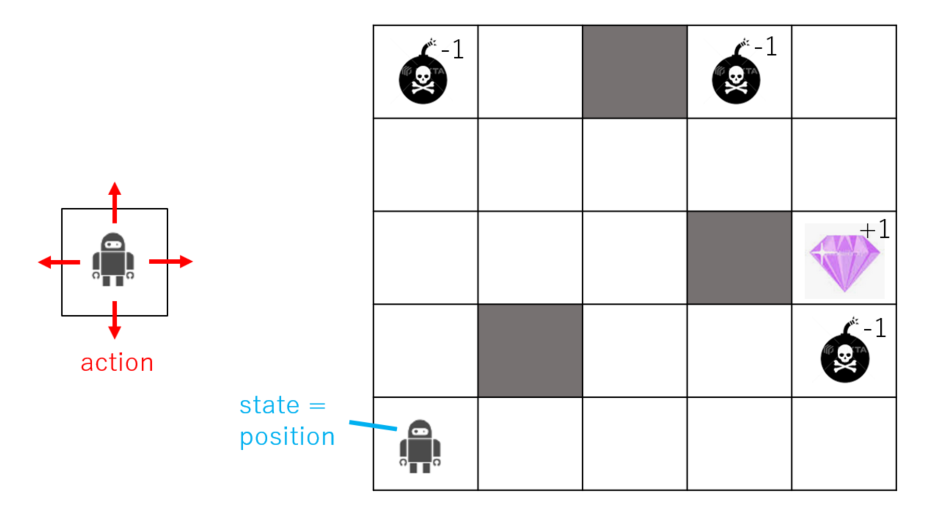
\includegraphics[width=14cm]{./figures/example_gridworld.png}
\caption{Grid world.}
\label{fig:example_gridworld}
\end{center}
\end{figure}

A Markov process that depends on a state in the past by one unit time is called a simple Markov process, and a Markov process that depends on a past state in more than two unit times is called a multiple Markov process. On the other hand, Markov processes that are not bound by past states are called homogeneous Markov processes. Here we concentrate on the homogeneous Markov process.


\subsection{Reinforcement learning problem formulation}

The problem of reinforcement learning can be formulated as a problem such that to find the optimal policy $\pi^{*}$ that maximizes the expected value of the time sum of rewards $R = \sum_{t'} \gamma^{t'} r_{t'+1}$ in the probability distribution $\pi(a|S_t,A_{t-1})$ that selects actions $a_t$ based on the realization values ​​of state time series $S_t = \{ s_1, ... , s_t\}$ and action time series $A_t = \{ a_1, ... , a_{t-1}\}$.

Here, $\gamma$ is the discount factor satisfying $0\leq \ \gamma \ \leq \ 1$, which is usually close to 1. (For example, $\gamma =1/(1+r)$ for some discount rate r.)
When the discount rate is applied, the sum of past rewards is evaluated lower than the latest reward.f the discount rate is not used, the sum of the rewards may diverge.

If dynamics of Markov decision process is homogeneous, then optimal homogeneous policy also exists.
If Markov model is homogeneous, the trajectory of the Agent $\bm{\zeta} = \{ (s_1, a_1), ... , (s_t, a_t) \}$ is generated by homogeneous dynamics $p(s'|s,a)$ and homogeneous policy$\pi(a|s)$.  


\begin{comment}
\subsection{Inverse reinforcement learning}

In general, designing an appropriate reward function is not easy. Inappropriate reward functions cause unintended behavior to the agent.
Although a precise calculation was required to design a reward function, it requires a great deal of human resources.
There is a new approach to solving the inverse problem of reinforcement learning to avoid designing reward functions.
Solving the inverse problem of reinforcement learning is called inverse reinforcement learning.

In inverse reinforcement learning, a sample of the behavior of the subject reinforcement learning problem expert is given, and the reward function that generated the sample is estimated.
Specifically, the trajectory sample $D = \{ \bm{\zeta}_1, ... ,\bm{\zeta}_n \}$ of an expert is given, and the inverse problem of estimating the reward function $r(s, a)$ that generated this sample is solved.

\begin{figure}[H]
\begin{center}
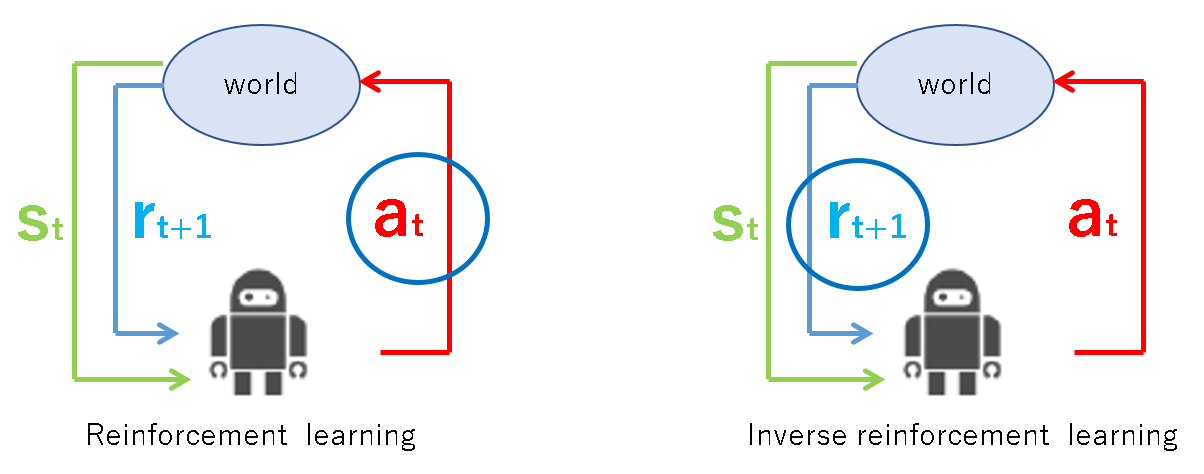
\includegraphics[width=11cm]{./figures/example_rl_irl.png}
\caption{Reinforcement learning focuses on improving the policy to make the at choice better. On the other hand, reverse reinforcement learning focuses on making the rewards more appropriate.}
\label{fig:example_rl_irl}
\end{center}
\end{figure}




\begin{itembox}[l]{"forward" reinforcement learning}
\bm{Given:} states $S$, actions $A$, dynamics $p(s,a)$, reword $R(s,a)$. \\
\bm{Find:} $\pi^* (a | s)$ 
\end{itembox}

\begin{itembox}[l]{inverse reinforcement learning}
\bm{Given:} states $S$, actions $A$, transitions $p(s,a)$, samples $D$ sampled from $\pi^*(D)$. \\
\bm{Find:} $R(s, a)$ 
\end{itembox}
\end{comment}

\subsection{Formulation of continuous state}


When discrete states and actions are considered, all reward function can be represented by a finite number.


\begin{figure}[H]
\begin{center}
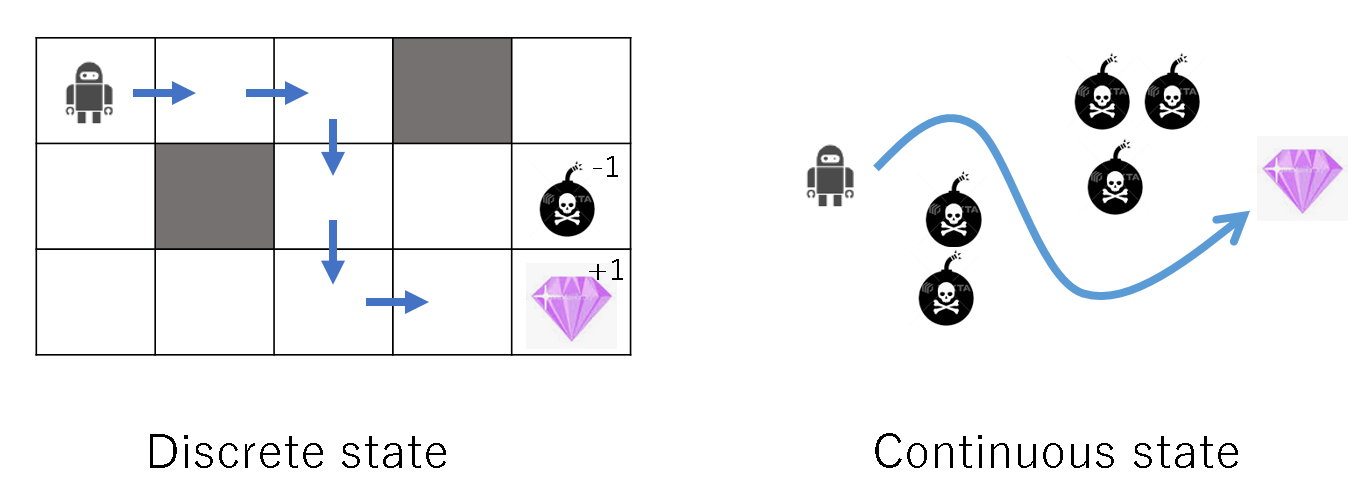
\includegraphics[width=11cm]{./figures/example_discrete_continuous.png}
\caption{Discrete state problem and continuous state problem.}
\label{fig:example_discrete_continuous}
\end{center}
\end{figure}


The state shown on the left side of the figure\ref{fig:example_discrete_continuous} has 13 positions and 4 actions, and then vector size of reword function is 52 $= 13 \times 4$.

\begin{itembox}[l]{grid world}

\bm{State space:} \hspace{1cm} $S = \{ s_1, s_2, ... , s_{13} \}$

\bm{Action:} \hspace{1.5cm} $A = \{ a_{up}, a_{right}, a_{left} , a_{down} \}$

\bm{Reword function:} $R = [ (s_1, a_{up}), (s_1, a_{right}), ... ,(s_{13}, a_{down}) ]^T$
\end{itembox}

For example, considering the state as shown on the right side of the figure\ref{fig:example_discrete_continuous}, this is considered to be a discrete problem in which the grid becomes extremely small.
In this case, the states increase without limit.
\begin{center}
State space: $S = [ s_0, s_1, ... ,s_{\infty} ]$
\end{center}
When we consider a situation where a set of positions are on $\mathbb{R}^2$, the reward function vector size will be infinite.
Here, the concept of a feature is newly introduced.

The feature is a value such as a gain for an trajectory. For example, the distance from trajectory to the nearest bomb can be called security, and it can also be called income based on whether or not agent can reach a treasure.
Then, the reward function can be redefined using the features as follows:
\[
R(s,a) = \theta_1 f_1(s,a) + \theta_2 f_2(s,a) + ... + \theta_n f_n(s,a).
\]
If the dimension of ${\bm \theta}$ is finite, the problem of specifying this coefficient is reduced to a problem of finite dimension.

Continuous state problems are often solved as a finite problem by introducing features. This report also introduces features.


\subsection{Action value function and State value function}

\begin{comment}
未来の報酬 R を最大化するために、将来の報酬の予測を表す関数、Q を定義する。
\end{comment}

To maximize future reward R, we define a action value function Q and state value function V that represents the forecast of future reward.

\[
V^{\pi}(s) = \mathbb{E}[R_{t} + \gamma R_{t+1} + \gamma^{2} R_{t+2}  + ....|s] = \mathbb{E} \Bigl[ \sum_{i=1}^{\infty} \gamma ^{i-1} R_{t+i} |s \Bigr]
\]

\[
Q^{\pi}(s,a) = \mathbb{E}[R_{t} + \gamma R_{t+1} + \gamma^{2} R_{t+2}  + ....|s,a] = \mathbb{E} \Bigl[ \sum_{i=1}^{\infty} \gamma ^{i-1} R_{t+i} |s,a \Bigr]
\]

\begin{comment}
方策πをπ'に更新する場合に、方策の更新のアドバンテージを評価するアドバンテージ関数を定義する。
\end{comment}

When updating the policy $\pi$ to $\pi′$, an advantage function that evaluates the advantage of updating the policy is defined.

\[
A^{\pi}(s,a) = Q^{\pi}(s,a) - V^{\pi}(s), \hspace{1cm} \forall (s,a) \in S \times A 
\]



\section{Introduction and formulation of generative adversarial imitation learning}

\subsection{Policy iteration}

\begin{comment}
将来の報酬の期待値を最大化するために、多くの手法が存在する。多くは価値反復か方策反復にカテゴライズされる。
価値反復は、初期価値関数Q0と最適方策を用意し、時間を1単位更新して価値関数Qtを更新する。方策反復は、適当な初期方策π0を用意して、方策評価Qπを求める。逐次方策を更新する。
\end{comment}

There are many approaches to maximizing expected future rewards. Many are categorized into value iterations or policy iterations.
In the value iteration, the initial value function $Q_0$ and the optimum policy are prepared, and the value function $Q_t$ is updated by updating the time by one unit. In the policy iteration, an appropriate initial policy $\pi_0$ is prepared and the policy evaluation $Q^{\pi_t}$ is obtained. Update policy sequentially.

\begin{comment}
状態が離散でなく連続の場合、行動の価値計算は容易でないため、方策反復の方が用いられる。本報告書は方策反復だけを述べる。
\end{comment}

When the state is continuous rather than discrete, value calculation of behavior is not easy, so policy iteration is used. This report describes only policy iterations.


\subsection{Policy gradient method}

\begin{comment}
確率方策を、関数近似する。
この関数を方策パラメータθについて微分し、勾配法を用いて学習することを考える。
\end{comment}

Function approximation of the stochastic policy.
Consider learning this function by differentiating it with respect to the policy parameter $\theta$.

\[
\theta' = \theta + \alpha \nabla_{\theta}\eta(\pi_\theta) , \hspace{5mm}
\Bigl( \eta(\theta) = V^{\pi_\theta}(s_t) = \sum_a \pi_\theta (a|s) Q^{\pi_\theta}(s,a) \Bigr)
\]

$\eta(\theta)$ is the expected gain and try to climb the gradient to maximize the expected gain.

\[
\nabla_\theta \eta(\theta)=\mathbb{E}\Bigl[ \nabla_\theta \log \pi_\theta(a|s) Q^{\pi_\theta}(s,a)   \Bigr]
\]

\[
\nabla_\theta \eta(\theta) \approx \sum_{t}^{T} \nabla_\theta \log (a_t|s_t)r_t
\]



\begin{figure}[H]
\begin{center}
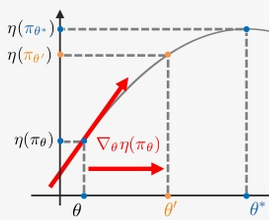
\includegraphics[width=5cm]{./figures/example_policy_gradient.png}
\caption{Policy gradient}
\label{fig:example_gridworld}
\end{center}
\end{figure}


\subsection{Introduction of Trust Region Policy Optimization(TRPO)}

\begin{comment}
方策をニューラルネットワークで実現する場合に、破壊的な操作が行われると回復することが出来なくなる。
それを回避するために、ニューラルネットの更新幅に制約を設けて、破壊的な更新が行われないように制限する方法が考えられる。
\end{comment}


When the policy is realized by a neural network, it cannot be recovered if a destructive operation is performed.
In order to avoid this, a method of limiting the update width of the neural network so that destructive update is not performed can be considered.

by {\it TRPO} (trust region policy optimization), $z$ is the ratio of policies $\pi_\theta$ and $\pi_{\theta'}$, and constraint on KL divergence of weight before and after update.

\[
z(\theta;s,a) = \frac{\pi_{\theta}(a|s)}{\pi_{\theta'}(a|s)}
\]

And thus, optimization formula is like as follows.

\begin{eqnarray*}
maximize ~\eta_{\mathrm{TRPO}}(\theta) = \underset{s,a}{\mathbb{E}}\Bigl[  z(\theta;s,a)A_{\theta}(s,a) \Bigr] \\
subject ~to~  \underset{s}{\mathbb{E}}\Bigl[ D_{\mathrm{KL}}(\pi_{\theta}(a|s)||\pi_{\theta'}(a|s)) \Bigr]  \leq \delta
\end{eqnarray*}


\subsection{Introduction of GAIL}

\begin{comment}
敵対的ネットワークは、強化学習を行う巧妙な手法である。この手法では、トレーニングのためのエキスパートによるデータがより少なくても効率的にエージェントを強化することが出来る。この手法では、強化エージェントの他に弁別器が用いられる。エージェントのポリシを進化させるのと同時に、弁別器はその行動がポリシのもたらしたものであるかエキスパートがもたらしたものであるか弁別する。

強化エージェントのポリシーと弁別器を同時に成長させることが特徴である。ポリシーは訓練が進むごとにより巧妙に弁別器をだまそうとする。その反対に弁別器はより巧妙に見破ろうとする。
\end{comment}

Adversarial networks are clever techniques for reinforcement learning. With this method, the agent can be effectively strengthened even if there is less data by the training expert. In this method, a discriminator is used in addition to the reinforcement agent. At the same time that the agent's policy is evolved, the discriminator discriminates whether the action is caused by the policy or by the expert.

The feature is to grow the policy of the strengthening agent and the discriminator at the same time. The policy tries to trick the discriminator more skillfully as the training progresses. On the contrary, the discriminator tries to detect it more subtly.\cite{HoE16}

Although $r(s_t,a_t)$ is unknown, a surrogate reward $\tilde{r}(s_t,a_t)$ may be learned directly from data, without making use of domain knowledge. 

Consider a set of simulated state-action pairs $\chi=(s_1,a_1),(s_2,a_2),...,(s_T,a_T)$ sampled from $\pi_\theta$ and a set of expert pairs $\chi_E$ sampled from $\pi_E$. 
For a neural network $D_\psi$ parameterized by $\psi$, the {\it GAIL} objective is given by:

\begin{eqnarray}
\underset{\psi}{\max}\hspace{1mm}
\underset{\theta}{\min}\hspace{1mm}
V(\theta, \psi) = 
\underset{(s,a) \sim \chi_E}{\mathbb{E}}[\log D_{\psi}] + 
\underset{(s,a) \sim \chi_{\theta}}{\mathbb{E}}[\log(1 - D_{\psi})] .
\label{equ:objective}
\end{eqnarray}

When fitting $\psi$, Equation \ref{equ:objective} can simply be interpreted as a sigmoid cross entropy objective, maximized by minibatch gradient ascent. 
Positive examples are sampled from $\chi_E$ and negative examples are sampled from rollouts generated by interactions of $\pi_\theta$ with the simulation environment. 
However, $V(\theta,\psi)$ is non-differentiable with respect to $\theta$, requiringoptimization via {\it RL}.
In order to fit $\pi_\theta$, a surrogate reward function can be formulated from Equation. \ref{equ:objective} as:

\begin{eqnarray}
\tilde{r}(s_t,a_t;\psi)=-\log (1-D_{\psi}(s_t,a_t)) ,
\end{eqnarray}

which approaches infinity as tuples $(s_t,a_t)$ drawn from $\chi_\theta$ become indistinguishable from elements of $\chi_E$ based on the predictions of $D_\psi$. 
After performing rollouts with a given set of policy parameters $\theta$, surrogate rewards $\tilde{r}(s_t,a_t;\psi)$ are calculated and {\it TRPO} is used to perform a policy update.
Although $\tilde{r}(s_t,a_t;\psi)$ may be quite different from the true reward function optimized by experts, it can be used to drive $\pi_\theta$ into regions of the state-action space similar to those explored by $\pi_E$.

